\chapter{Experiments}

\section{Method}

We conducted experiments over three type of functions: the \texttt{Cata Sum}, \texttt{Generic Cata Sum} and \texttt{Incremental Cata Sum}. The Cata Sum is the simple function which traverses through the entire tree and sums all the values. The Generic Cata Sum is the initial Incremental Cata Sum, which starts with an empty HashMap. And the Incremental Cata Sum, which already has a HashMap filled with cached results and keeps track over multiple iterations.

\begin{minted}{haskell}
cataSum :: Tree Int -> Int
cataSum (Leaf x)     = x
cataSum (Node l x r) = x + cataSum l + cataSum r

genericCataSum :: Merkle (PF (Tree Int)) -> (Int, HashMap Digest Int)
genericCataSum = cataMerkle
  (\case
    Leaf_ x     -> x
    Node_ l x r -> l + x + r
  )

incCataSum :: HashMap Digest Int 
           -> Merkle (PF (Tree Int)) -> (Int, HashMap Digest Int)
incCataSum = cataMerkleMap
  (\case
    Leaf_ x     -> x
    Node_ l x r -> l + x + r
  )
\end{minted}

The experiments will be benchmarks executed with the Haskell package \texttt{criterion}\cite{hackage2022criterion}. Criterion performs the benchmarks multiple times to get an average result. The benchmarks will track two metrics: the \textit{execution time} and the \textit{memory usage}. The execution time will be in seconds and the memory usage will be the max-bytes used. The results gathered for the execution time comes from the criterion package, however the memory usage will not come from the package. This is because criterion only keeps track of the memory allocation and not usage. Therefore, we measure the memory usage with the GHC profiler\cite*{ghc2022memoryprofiling} and profile every benchmark individually to know its memory usage.

To test how well the three functions perform, we perform three types of updates, multiple times. These benchmarks will be based on the three type of cases: worst, average and best. The worst case updates the lowest left leaf with a new leaf. The average case updates a node in the middle of the data structure with a new leaf. And the best case updates the left child of the root-node with a new leaf.

\begin{minted}{haskell}
worstCase :: Merkle (PF (Tree Int)) -> Merkle (PF (Tree Int))
worstCase = update (const (Leaf i)) [Bttm]

averageCase :: Merkle (PF (Tree Int)) -> Merkle (PF (Tree Int))
averageCase = update (const (Leaf i)) (replicate n Dwn)
  where
    n = round (logBase 2.0 (fromIntegral n) / 2.0)

bestCase :: Merkle (PF (Tree Int)) -> Merkle (PF (Tree Int))
bestCase = update (const (Leaf i)) [Dwn]
\end{minted}

\section{Results}

The experiments are performed on a laptop with a \texttt{Intel Core i7-8750H} with a base clock of \texttt{2.2GHz} and a boost clock of \texttt{4.1GHz}, with \texttt{16GB} of memory. First we explain the results of the three algorithms with three different scenarios, iterating 10 times. Then, we show the results of adding a cache addition policy. The code used for the benchmarks can be found at: \href{https://github.com/jortvangorkum/memo-cata}{\texttt{https://github.com/jortvangorkum/memo-cata}}

\subsection{Execution Time}
Looking at \Cref{fig-exec-time-no-policy} the Incremental Cata Sum is faster when the tree contains more than $10^3$ nodes. However, for every benchmark the execution time is better or worse depending on the type of update that is performed. The best case scenario has the biggest difference, then the average case and the closest execution time difference is the worst case. The execution time for Cata Sum and Generic Cata Sum seems to be linear with the amount of nodes and the Incremental Cata Sum is constant/logarithmic. The Cata Sum seems to be a factor faster than the Generic Cata Sum, which makes sense because Generic Cata Sum does the same computation as the Cata Sum. And, additionally computes the generic representation of the data structure, computes the digests for the data structure and stores all the cached result into a \texttt{HashMap}. The Incremental Cata Sum is constant/logarithmic, because it only updates the digests of the changed nodes and its parent nodes and recomputes the nodes with changed digests, which is worst case $\mathcal{O}(M \log{N})$ where $M$ is the amount of changes and $N$ is the size of the tree. The discrepancy in the range between $10^2 - 10^3$ is probably because the amount of nodes is too low to get stable results.

\begin{figure}[H]
  \begin{minipage}{.5\textwidth}
    \centering
    \includegraphics[width=\textwidth]{plots/run-3/time/Worst/10/all_benchmarks.pdf}
  \end{minipage}
  \begin{minipage}{.5\textwidth}
    \centering
    \includegraphics[width=\textwidth]{plots/run-3/time/Average/10/all_benchmarks.pdf}  
  \end{minipage}
  \begin{center}
    \begin{minipage}[c]{.5\textwidth}
      \centering
      \includegraphics[width=\textwidth]{plots/run-3/time/Best/10/all_benchmarks.pdf}  
    \end{minipage}
  \end{center}
  \caption{The execution time over 10 executions for the Worst, Average and Best case.}
  \label{fig-exec-time-no-policy}
\end{figure}

\subsection{Memory Usage}
The \Cref*{fig-mem-usage-no-policy} shows that the memory usage is, for all algorithms, linear with the amount of nodes. The Cata Sum uses the least amount of memory, then the Incremental Cata Sum and the most used bytes is the Generic Cata Sum. We think that the Incremental Cata Sum uses less memory than the Generic Cata Sum, because the Incremental Cata Sum needs to load-in fewer parts of the data structure than the Generic Cata Sum. Also, the same discrepancy occurs in the range between $10^2 - 10^3$ as with the execution time.

\begin{figure}[H]
  \begin{minipage}{.5\textwidth}
    \centering
    \includegraphics[width=\textwidth]{plots/run-3/memory/Worst/10/all_benchmarks.pdf}  
  \end{minipage}
  \begin{minipage}{.5\textwidth}
    \centering
    \includegraphics[width=\textwidth]{plots/run-3/memory/Average/10/all_benchmarks.pdf}  
  \end{minipage}
  \begin{center}
    \begin{minipage}[c]{.5\textwidth}
      \centering
      \includegraphics[width=\textwidth]{plots/run-3/memory/Best/10/all_benchmarks.pdf}  
    \end{minipage}
  \end{center}
  \caption{The max-bytes-used over 10 executions for the Worst, Average and Best case.}
  \label{fig-mem-usage-no-policy}
\end{figure}

\subsection{Comparison Cache Addition Policies}

As seen in \Cref*{fig-exec-time-policy-rec-depth-5} and \Cref*{fig-mem-usage-policy-rec-depth-5}, the memory usage is lower than when all the cached results are stored. Even, the execution time did not increase significantly. However, this is probably because the function which is computed (addition) is not computational intensive. This means it is less computational intensive to recompute the value than to store the value and retrieve it when needed. This does not have to be the case for more extensive computations. So, for the best performance this parameter needs to be correctly tweaked.

For example, if we increased the recursion depth limit to 10. The results in Appendix Section \ref*{app-sec-10-rec-depth} show that the memory usage is even lower than the limit of 5. However, the execution time increases significantly. This is because the computation takes longer to perform than to store and perform a lookup. 

\subsection*{Execution Time}
\begin{figure}[H]
  \begin{minipage}{.5\textwidth}
    \centering
    \includegraphics[width=\textwidth]{plots/run-4/time/Worst/10/all_benchmarks.pdf}  
  \end{minipage}
  \begin{minipage}{.5\textwidth}
    \centering
    \includegraphics[width=\textwidth]{plots/run-4/time/Average/10/all_benchmarks.pdf}  
  \end{minipage}
  \begin{center}
    \begin{minipage}[c]{.5\textwidth}
      \centering
      \includegraphics[width=\textwidth]{plots/run-4/time/Best/10/all_benchmarks.pdf}  
    \end{minipage}
  \end{center}
  \caption{The execution time over 10 executions for the Worst, Average and Best case, where the minimum recursion depth is 5.}
  \label{fig-exec-time-policy-rec-depth-5}
\end{figure}

\subsection*{Memory Usage}
\begin{figure}[H]
  \begin{minipage}{.5\textwidth}
    \centering
    \includegraphics[width=\textwidth]{plots/run-4/memory/Worst/10/all_benchmarks.pdf}  
  \end{minipage}
  \begin{minipage}{.5\textwidth}
    \centering
    \includegraphics[width=\textwidth]{plots/run-4/memory/Average/10/all_benchmarks.pdf}  
  \end{minipage}
  \begin{center}
    \begin{minipage}[c]{.5\textwidth}
      \centering
      \includegraphics[width=\textwidth]{plots/run-4/memory/Best/10/all_benchmarks.pdf}  
    \end{minipage}
  \end{center}
  \caption{The max-bytes-used over 10 executions for the Worst, Average and Best case, where the minimum recursion depth is 5.}
  \label{fig-mem-usage-policy-rec-depth-5}
\end{figure}
